\documentclass{article}
\usepackage{tikz}
\usetikzlibrary{positioning, arrows.meta, fit, backgrounds}

\begin{document}
\pagecolor{black}
\pagestyle{empty}
\color{white}
\definecolor{green}{HTML}{52753d}
\definecolor{red}{HTML}{873839}
\definecolor{purple}{HTML}{644475}
\definecolor{gray}{HTML}{595959}
\definecolor{blue}{HTML}{42538b}
\definecolor{cyan}{HTML}{328486}
\definecolor{orange}{HTML}{e09166}

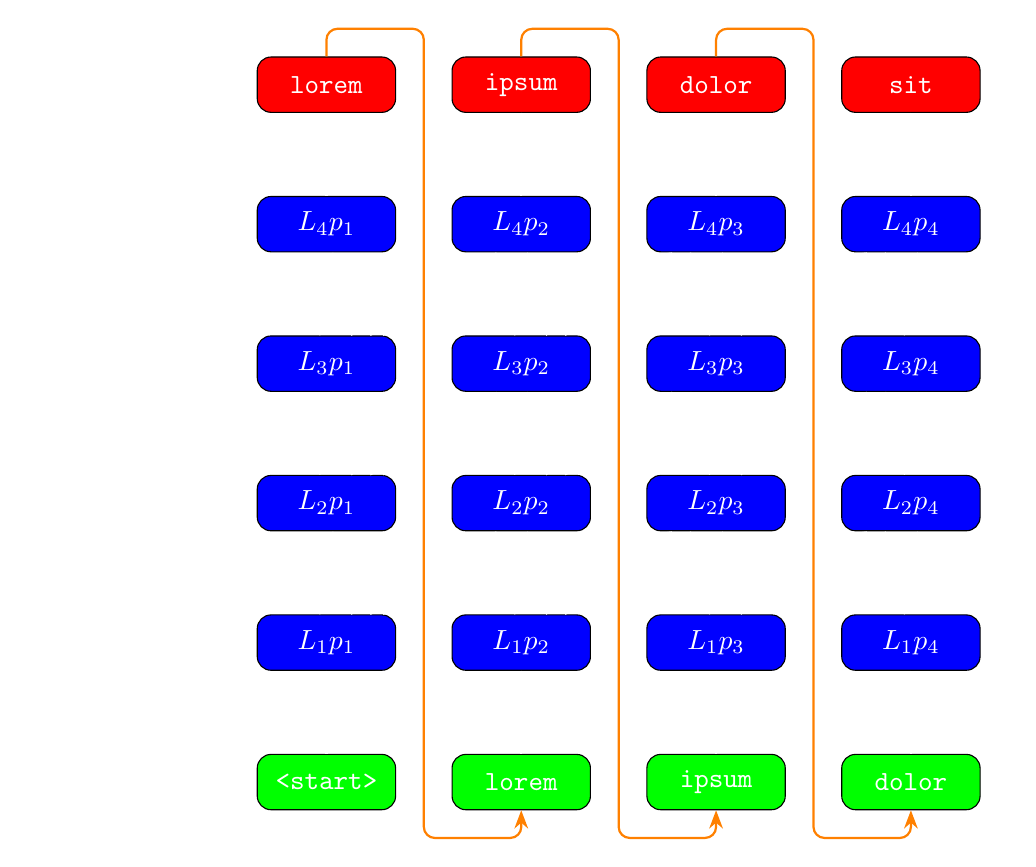
\begin{tikzpicture}[node distance=30pt and 20pt, >=Stealth,
    every node/.style={draw=black, minimum width=50pt, minimum height=20pt, align=center, rounded corners=5pt, text=white},
    input/.style={fill=green},
    output/.style={fill=red},
    hidden/.style={fill=blue},
    attention/.style={->, draw=white, bend left},
    recurrence/.style={->, draw=orange, thick, rounded corners},
    phantom/.style={->, draw=white, thick, dashed},
    ]

% \begin{tikzpicture}[node distance=30pt and 20pt, >=Stealth, thick,
%     every node/.style={draw, minimum width=50pt, minimum height=20pt, align=center, rounded corners=5pt},
%     input/.style={fill=green!20},
%     output/.style={fill=red!20},
%     hidden/.style={fill=gray!20},
%     attention/.style={->, draw=black!70, thick, bend left},
%     recurrence/.style={->, draw=blue!70, thick, rounded corners},
%     phantom/.style={->, draw=black, thick, dashed},
%     ]

% Nodes for input layer
\begin{scope}[local bounding box=input box]
    \node[input] (x1) {\tt{<start>}};
    \node[input, right=of x1] (x2) {\tt{lorem}};
    \node[input, right=of x2] (x3) {\tt{ipsum}};
    \node[input, right=of x3] (x4) {\tt{dolor}};
\end{scope}
\node[fit=(input box), draw=none, label=left:Input Tokens, inner sep=10pt] {};

% Nodes for hidden layer L1
\begin{scope}[local bounding box=l1 box]
    \node[hidden, above=of x1] (l1h1) {$L_{1}p_1$};
    \node[hidden, right=of l1h1] (l1h2) {$L_{1}p_2$};
    \node[hidden, right=of l1h2] (l1h3) {$L_{1}p_3$};
    \node[hidden, right=of l1h3] (l1h4) {$L_{1}p_4$};
\end{scope}
\node[fit=(l1 box), draw=none, label=left:$L_1$, inner sep=10pt] {};

% Nodes for hidden layer L2
\begin{scope}[local bounding box=l2 box]
    \node[hidden, above=of l1h1] (l2h1) {$L_{2}p_1$};
    \node[hidden, right=of l2h1] (l2h2) {$L_{2}p_2$};
    \node[hidden, right=of l2h2] (l2h3) {$L_{2}p_3$};
    \node[hidden, right=of l2h3] (l2h4) {$L_{2}p_4$};
\end{scope}
\node[fit=(l2 box), draw=none, label=left:$L_2$, inner sep=10pt] {};

% Nodes for hidden layer L3
\begin{scope}[local bounding box=l3 box]
    \node[hidden, above=of l2h1] (l3h1) {$L_{3}p_1$};
    \node[hidden, right=of l3h1] (l3h2) {$L_{3}p_2$};
    \node[hidden, right=of l3h2] (l3h3) {$L_{3}p_3$};
    \node[hidden, right=of l3h3] (l3h4) {$L_{3}p_4$};
\end{scope}
\node[fit=(l3 box), draw=none, label=left:$L_3$, inner sep=10pt] {};

% Nodes for hidden layer L4
\begin{scope}[local bounding box=l4 box]
    \node[hidden, above=of l3h1] (l4h1) {$L_{4}p_1$};
    \node[hidden, right=of l4h1] (l4h2) {$L_{4}p_2$};
    \node[hidden, right=of l4h2] (l4h3) {$L_{4}p_3$};
    \node[hidden, right=of l4h3] (l4h4) {$L_{4}p_4$};
\end{scope}
\node[fit=(l4 box), draw=none, label=left:$L_4$, inner sep=10pt] {};

% Ellipsis node
% \node[above=of l4 box, align=center, draw=none] (ellipsis) {\vdots};

% Nodes for output layer
\begin{scope}[local bounding box=output box]
    \node[output, above=of l4h1] (y1) {\tt{lorem}};
    \node[output, right=of y1] (y2) {\tt{ipsum}};
    \node[output, right=of y2] (y3) {\tt{dolor}};
    \node[output, right=of y3] (y4) {\tt{sit}};
\end{scope}
\node[fit=(output box), draw=none, label=left:Output Tokens, inner sep=10pt] {};

% input tokens to L1
\draw[phantom] (x1) -- (l1h1);
\draw[phantom] (x2) -- (l1h2);
\draw[phantom] (x3) -- (l1h3);
\draw[phantom] (x4) -- (l1h4);

% attention connections from L1 to L2
\draw[attention] (l1h1) to[out=13, in=193] (l2h1);
\draw[attention] (l1h2) to[out=13, in=193] (l2h2);
\draw[attention] (l1h3) to[out=13, in=193] (l2h3);
\draw[attention] (l1h4) to[out=13, in=193] (l2h4);
\draw[attention] (l1h1) to[out=13, in=193] (l2h2);
\draw[attention] (l1h1) to[out=13, in=193] (l2h3);
\draw[attention] (l1h1) to[out=13, in=193] (l2h4);
\draw[attention] (l1h2) to[out=13, in=193] (l2h3);
\draw[attention] (l1h2) to[out=13, in=193] (l2h4);
\draw[attention] (l1h3) to[out=13, in=193] (l2h4);

% attention connections from L2 to L3
\draw[attention] (l2h1) to[out=13, in=193] (l3h1);
\draw[attention] (l2h2) to[out=13, in=193] (l3h2);
\draw[attention] (l2h3) to[out=13, in=193] (l3h3);
\draw[attention] (l2h4) to[out=13, in=193] (l3h4);
\draw[attention] (l2h1) to[out=13, in=193] (l3h2);
\draw[attention] (l2h1) to[out=13, in=193] (l3h3);
\draw[attention] (l2h1) to[out=13, in=193] (l3h4);
\draw[attention] (l2h2) to[out=13, in=193] (l3h3);
\draw[attention] (l2h2) to[out=13, in=193] (l3h4);
\draw[attention] (l2h3) to[out=13, in=193] (l3h4);

% attention connections from L3 to L4
\draw[attention] (l3h1) to[out=13, in=193] (l4h1);
\draw[attention] (l3h2) to[out=13, in=193] (l4h2);
\draw[attention] (l3h3) to[out=13, in=193] (l4h3);
\draw[attention] (l3h4) to[out=13, in=193] (l4h4);
\draw[attention] (l3h1) to[out=13, in=193] (l4h2);
\draw[attention] (l3h1) to[out=13, in=193] (l4h3);
\draw[attention] (l3h1) to[out=13, in=193] (l4h4);
\draw[attention] (l3h2) to[out=13, in=193] (l4h3);
\draw[attention] (l3h2) to[out=13, in=193] (l4h4);
\draw[attention] (l3h3) to[out=13, in=193] (l4h4);

% final hidden layer to output tokens
\draw[phantom] (l4h1) -- (y1);
\draw[phantom] (l4h2) -- (y2);
\draw[phantom] (l4h3) -- (y3);
\draw[phantom] (l4h4) -- (y4);

% autoregressive recurrence

% Draw the recurrence connections with waypoints
\node[coordinate, above right=10pt and 10pt of y1] (p1o) {};
\node[coordinate, below left =10pt and 10pt of x2] (p1i) {};
\draw[recurrence] (y1.north) |- (p1o) -- (p1i) -| (x2.south);

\node[coordinate, above right=10pt and 10pt of y2] (p2o) {};
\node[coordinate, below left =10pt and 10pt of x3] (p2i) {};
\draw[recurrence] (y2.north) |- (p2o) -- (p2i) -| (x3.south);

\node[coordinate, above right=10pt and 10pt of y3] (p3o) {};
\node[coordinate, below left =10pt and 10pt of x4] (p3i) {};
\draw[recurrence] (y3.north) |- (p3o) -- (p3i) -| (x4.south);

\end{tikzpicture}
\end{document}
